\documentclass[tikz,border=0pt]{standalone}
\usepackage{xcolor}
\usetikzlibrary{calc}
% Palette: Sam_Comm_final.png by eye, and the drones and raiders.
\definecolor{ink}{HTML}{3B2340}
\definecolor{sky}{HTML}{EFC46A}
\definecolor{skyhi}{HTML}{F5DA92}
\definecolor{skylow}{HTML}{E9B060}
\definecolor{cloud}{HTML}{F2D58A}
\definecolor{paper}{HTML}{FBEFD0}
\definecolor{cream}{HTML}{FFF6E0}
\definecolor{white}{HTML}{FFFFFF}
\definecolor{wallA}{HTML}{E88A73}
\definecolor{wallB}{HTML}{EE9F7E}
\definecolor{wallC}{HTML}{E47A7E}
\definecolor{wallD}{HTML}{F0B07E}
\definecolor{wallE}{HTML}{D9765F}
\definecolor{wallF}{HTML}{E99A8A}
\definecolor{greenA}{HTML}{8DBB7E}
\definecolor{greenB}{HTML}{6FA77A}
\definecolor{greenC}{HTML}{A9C97F}
\definecolor{greenD}{HTML}{5E9C6A}
\definecolor{greenE}{HTML}{4A8060}
\definecolor{sage}{HTML}{9DB98A}
\definecolor{sagedark}{HTML}{6F8F66}
\definecolor{sagelight}{HTML}{C2D6A6}
\definecolor{window}{HTML}{F6E7A0}
\definecolor{windark}{HTML}{8C5A64}
\definecolor{metal}{HTML}{8D9A93}
\definecolor{metaldark}{HTML}{5E6B66}
\definecolor{metallight}{HTML}{B9C4BC}
\definecolor{wood}{HTML}{B9835A}
\definecolor{wooddark}{HTML}{8C5A3C}
\definecolor{woodlight}{HTML}{D9A66F}
\definecolor{stone}{HTML}{E7C9A0}
\definecolor{stonedark}{HTML}{C9A47E}
\definecolor{concrete}{HTML}{D8C3A4}
\definecolor{concretedark}{HTML}{B8A084}
\definecolor{asphalt}{HTML}{8E7A86}
\definecolor{asphaltdark}{HTML}{6E5C68}
\definecolor{roadline}{HTML}{F6E7A0}
\definecolor{kerb}{HTML}{D8B48C}
\definecolor{red}{HTML}{E0483E}
\definecolor{redlight}{HTML}{F27A6A}
\definecolor{gold}{HTML}{FFB000}
\definecolor{goldlight}{HTML}{FFD54F}
\definecolor{teal}{HTML}{4FA3A0}
\definecolor{tealdark}{HTML}{3C8582}
\definecolor{magenta}{HTML}{FF2E88}
\definecolor{cyan}{HTML}{13CFE3}
\definecolor{violet}{HTML}{8A5BD6}
\definecolor{orange}{HTML}{F2803A}
\definecolor{pink}{HTML}{F48FB1}
\definecolor{glow}{HTML}{4FE6E0}
\definecolor{glowhi}{HTML}{C8FFF9}
\definecolor{hot}{HTML}{FF6A1A}
\definecolor{hothi}{HTML}{FFD07A}
\definecolor{armour}{HTML}{7E7A86}
\definecolor{armourdark}{HTML}{5A5466}
\definecolor{armourlight}{HTML}{A8A2B0}
\definecolor{wasp}{HTML}{E0A82E}
\definecolor{waspdark}{HTML}{B07E1A}
\definecolor{moth}{HTML}{F2E6C8}
\definecolor{mothdark}{HTML}{D2C09A}
\definecolor{hornet}{HTML}{3C8582}
\definecolor{hornetdark}{HTML}{2C6260}
\definecolor{warden}{HTML}{E47A7E}
\definecolor{wardendark}{HTML}{B85A62}
\definecolor{tick}{HTML}{8DBB7E}
\definecolor{tickdark}{HTML}{5E8A5A}
\definecolor{strider}{HTML}{D9765F}
\definecolor{striderdark}{HTML}{A8543F}
\definecolor{jacket}{HTML}{6FA77A}
\definecolor{jacketb}{HTML}{4FA3A0}
\definecolor{jacketc}{HTML}{E88A73}
\definecolor{jacketd}{HTML}{F0B07E}
\definecolor{skin}{HTML}{F2C49A}
\definecolor{skinb}{HTML}{C98C6A}
\definecolor{skinc}{HTML}{8C5A3C}
\definecolor{hair}{HTML}{3B2340}
\definecolor{goo}{HTML}{B6E35A}
\definecolor{goodark}{HTML}{7FB23A}
\newcommand{\Ink}{1.8pt}
\tikzset{inked/.style={draw=ink, line width=\Ink, line join=round, line cap=round}}
\begin{document}
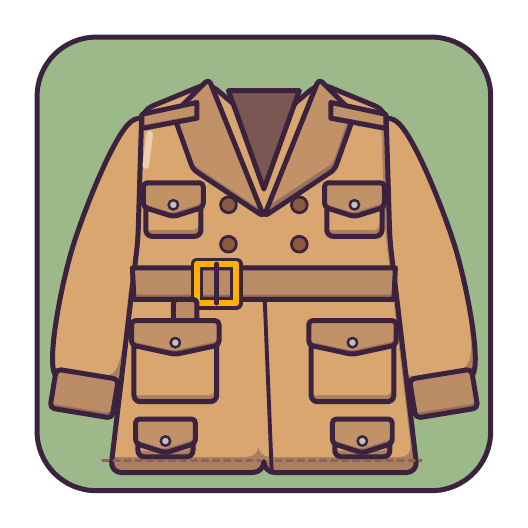
\begin{tikzpicture}
\clip (0,0) rectangle (6,6);
\fill[sage] [rounded corners=0.75cm] (0.12,0.12) rectangle (5.88,5.88);
\begin{scope}\clip [rounded corners=0.75cm] (0.12,0.12) rectangle (5.88,5.88);
\begin{scope}\clip plot[smooth cycle, tension=0.5] coordinates {(4.681,4.812) (5.428,3.215) (5.664,1.618) (4.836,1.482) (4.572,2.935) (3.819,4.388)};
\fill[woodlight!70!ink] plot[smooth cycle, tension=0.5] coordinates {(4.681,4.812) (5.428,3.215) (5.664,1.618) (4.836,1.482) (4.572,2.935) (3.819,4.388)};
\fill[woodlight, shift={(-0.056,0.16)}] plot[smooth cycle, tension=0.5] coordinates {(4.681,4.812) (5.428,3.215) (5.664,1.618) (4.836,1.482) (4.572,2.935) (3.819,4.388)};
\end{scope}
\draw[inked] plot[smooth cycle, tension=0.5] coordinates {(4.681,4.812) (5.428,3.215) (5.664,1.618) (4.836,1.482) (4.572,2.935) (3.819,4.388)};
\begin{scope}\clip[rounded corners=0.06cm] (5.636,1.664) -- (5.717,1.17) -- (4.929,1.041) -- (4.848,1.535) -- cycle;
\fill[woodlight!80!ink!70!ink,rounded corners=0.06cm] (5.636,1.664) -- (5.717,1.17) -- (4.929,1.041) -- (4.848,1.535) -- cycle;
\fill[woodlight!80!ink,rounded corners=0.06cm, shift={(-0.021,0.06)}] (5.636,1.664) -- (5.717,1.17) -- (4.929,1.041) -- (4.848,1.535) -- cycle;
\end{scope}
\draw[inked,rounded corners=0.06cm] (5.636,1.664) -- (5.717,1.17) -- (4.929,1.041) -- (4.848,1.535) -- cycle;
\begin{scope}\clip plot[smooth cycle, tension=0.5] coordinates {(2.181,4.388) (1.428,2.935) (1.164,1.482) (0.336,1.618) (0.572,3.215) (1.319,4.812)};
\fill[woodlight!70!ink] plot[smooth cycle, tension=0.5] coordinates {(2.181,4.388) (1.428,2.935) (1.164,1.482) (0.336,1.618) (0.572,3.215) (1.319,4.812)};
\fill[woodlight, shift={(-0.056,0.16)}] plot[smooth cycle, tension=0.5] coordinates {(2.181,4.388) (1.428,2.935) (1.164,1.482) (0.336,1.618) (0.572,3.215) (1.319,4.812)};
\end{scope}
\draw[inked] plot[smooth cycle, tension=0.5] coordinates {(2.181,4.388) (1.428,2.935) (1.164,1.482) (0.336,1.618) (0.572,3.215) (1.319,4.812)};
\begin{scope}\clip[rounded corners=0.06cm] (1.152,1.535) -- (1.071,1.041) -- (0.283,1.17) -- (0.364,1.664) -- cycle;
\fill[woodlight!80!ink!70!ink,rounded corners=0.06cm] (1.152,1.535) -- (1.071,1.041) -- (0.283,1.17) -- (0.364,1.664) -- cycle;
\fill[woodlight!80!ink,rounded corners=0.06cm, shift={(-0.021,0.06)}] (1.152,1.535) -- (1.071,1.041) -- (0.283,1.17) -- (0.364,1.664) -- cycle;
\end{scope}
\draw[inked,rounded corners=0.06cm] (1.152,1.535) -- (1.071,1.041) -- (0.283,1.17) -- (0.364,1.664) -- cycle;
\begin{scope}\clip [rounded corners=0.14cm] (3,4.7) -- (3.7,5.3) -- (4.55,4.95) -- (4.6,3.3) -- (4.95,0.35) -- (3,0.35) -- (3,0.35) -- (1.05,0.35) -- (1.4,3.3) -- (1.45,4.95) -- (2.3,5.3) -- (3,4.7) -- cycle;
\fill[woodlight!70!ink] [rounded corners=0.14cm] (3,4.7) -- (3.7,5.3) -- (4.55,4.95) -- (4.6,3.3) -- (4.95,0.35) -- (3,0.35) -- (3,0.35) -- (1.05,0.35) -- (1.4,3.3) -- (1.45,4.95) -- (2.3,5.3) -- (3,4.7) -- cycle;
\fill[woodlight, shift={(-0.07,0.2)}] [rounded corners=0.14cm] (3,4.7) -- (3.7,5.3) -- (4.55,4.95) -- (4.6,3.3) -- (4.95,0.35) -- (3,0.35) -- (3,0.35) -- (1.05,0.35) -- (1.4,3.3) -- (1.45,4.95) -- (2.3,5.3) -- (3,4.7) -- cycle;
\end{scope}
\draw[inked] [rounded corners=0.14cm] (3,4.7) -- (3.7,5.3) -- (4.55,4.95) -- (4.6,3.3) -- (4.95,0.35) -- (3,0.35) -- (3,0.35) -- (1.05,0.35) -- (1.4,3.3) -- (1.45,4.95) -- (2.3,5.3) -- (3,4.7) -- cycle;
\draw[ink, line width=1.4pt, line cap=round] (3,2.8) -- (3.1,0.35);
\begin{scope}\clip[rounded corners=0.06cm] (3,3.6) -- (2.3,5.35) -- (1.85,4.9) -- (2.1,4.2) -- cycle;
\fill[woodlight!85!ink!70!ink,rounded corners=0.06cm] (3,3.6) -- (2.3,5.35) -- (1.85,4.9) -- (2.1,4.2) -- cycle;
\fill[woodlight!85!ink,rounded corners=0.06cm, shift={(-0.028,0.08)}] (3,3.6) -- (2.3,5.35) -- (1.85,4.9) -- (2.1,4.2) -- cycle;
\end{scope}
\draw[inked,rounded corners=0.06cm] (3,3.6) -- (2.3,5.35) -- (1.85,4.9) -- (2.1,4.2) -- cycle;
\begin{scope}\clip[rounded corners=0.06cm] (3,3.6) -- (3.7,5.35) -- (4.15,4.9) -- (3.9,4.2) -- cycle;
\fill[woodlight!85!ink!70!ink,rounded corners=0.06cm] (3,3.6) -- (3.7,5.35) -- (4.15,4.9) -- (3.9,4.2) -- cycle;
\fill[woodlight!85!ink,rounded corners=0.06cm, shift={(-0.028,0.08)}] (3,3.6) -- (3.7,5.35) -- (4.15,4.9) -- (3.9,4.2) -- cycle;
\end{scope}
\draw[inked,rounded corners=0.06cm] (3,3.6) -- (3.7,5.35) -- (4.15,4.9) -- (3.9,4.2) -- cycle;
\filldraw[inked, fill=woodlight!40!ink] (2.55,5.2) -- (3.45,5.2) -- (3.0,3.95) -- cycle;
\begin{scope}\clip (2.15,5.05) -- (1.45,4.9) -- (1.45,4.72) -- (2.15,4.85) -- cycle;
\fill[woodlight!85!ink!70!ink] (2.15,5.05) -- (1.45,4.9) -- (1.45,4.72) -- (2.15,4.85) -- cycle;
\fill[woodlight!85!ink, shift={(-0.014,0.04)}] (2.15,5.05) -- (1.45,4.9) -- (1.45,4.72) -- (2.15,4.85) -- cycle;
\end{scope}
\draw[inked] (2.15,5.05) -- (1.45,4.9) -- (1.45,4.72) -- (2.15,4.85) -- cycle;
\begin{scope}\clip (3.85,5.05) -- (4.55,4.9) -- (4.55,4.72) -- (3.85,4.85) -- cycle;
\fill[woodlight!85!ink!70!ink] (3.85,5.05) -- (4.55,4.9) -- (4.55,4.72) -- (3.85,4.85) -- cycle;
\fill[woodlight!85!ink, shift={(-0.014,0.04)}] (3.85,5.05) -- (4.55,4.9) -- (4.55,4.72) -- (3.85,4.85) -- cycle;
\end{scope}
\draw[inked] (3.85,5.05) -- (4.55,4.9) -- (4.55,4.72) -- (3.85,4.85) -- cycle;
\filldraw[inked,fill=wooddark,line width=1.0pt] (2.55,3.75) circle (0.1);
\filldraw[inked,fill=wooddark,line width=1.0pt] (3.45,3.75) circle (0.1);
\filldraw[inked,fill=wooddark,line width=1.0pt] (2.55,3.25) circle (0.1);
\filldraw[inked,fill=wooddark,line width=1.0pt] (3.45,3.25) circle (0.1);
\begin{scope}\clip (1.35,2.55) -- (4.65,2.55) -- (4.67,2.95) -- (1.33,2.95) -- cycle;
\fill[woodlight!80!ink!70!ink] (1.35,2.55) -- (4.65,2.55) -- (4.67,2.95) -- (1.33,2.95) -- cycle;
\fill[woodlight!80!ink, shift={(-0.021,0.06)}] (1.35,2.55) -- (4.65,2.55) -- (4.67,2.95) -- (1.33,2.95) -- cycle;
\end{scope}
\draw[inked] (1.35,2.55) -- (4.65,2.55) -- (4.67,2.95) -- (1.33,2.95) -- cycle;
\draw[ink, line width=4.6pt, line join=round] (2.15,2.5) -- (2.65,2.5) -- (2.65,3) -- (2.15,3) -- cycle;
\draw[gold, line width=2.2pt, line join=round] (2.15,2.5) -- (2.65,2.5) -- (2.65,3) -- (2.15,3) -- cycle;
\draw[ink, line width=1.6pt, line cap=round] (2.4,2.5) -- (2.4,3);
\begin{scope}\clip[rounded corners=0.05cm] (1.85,1.95) rectangle (2.15,2.55);
\fill[woodlight!80!ink!70!ink,rounded corners=0.05cm] (1.85,1.95) rectangle (2.15,2.55);
\fill[woodlight!80!ink,rounded corners=0.05cm, shift={(-0.01,0.03)}] (1.85,1.95) rectangle (2.15,2.55);
\end{scope}
\draw[inked,rounded corners=0.05cm] (1.85,1.95) rectangle (2.15,2.55);
\begin{scope}\clip[rounded corners=0.08cm] (1.5,3.35) rectangle (2.2,4);
\fill[woodlight!70!ink,rounded corners=0.08cm] (1.5,3.35) rectangle (2.2,4);
\fill[woodlight,rounded corners=0.08cm, shift={(-0.028,0.08)}] (1.5,3.35) rectangle (2.2,4);
\end{scope}
\draw[inked,rounded corners=0.08cm] (1.5,3.35) rectangle (2.2,4);
\begin{scope}\clip[rounded corners=0.05cm] (1.47,4.03) -- (2.23,4.03) -- (2.23,3.72) -- (1.85,3.6) -- (1.47,3.72) -- cycle;
\fill[woodlight!85!ink!70!ink,rounded corners=0.05cm] (1.47,4.03) -- (2.23,4.03) -- (2.23,3.72) -- (1.85,3.6) -- (1.47,3.72) -- cycle;
\fill[woodlight!85!ink,rounded corners=0.05cm, shift={(-0.017,0.05)}] (1.47,4.03) -- (2.23,4.03) -- (2.23,3.72) -- (1.85,3.6) -- (1.47,3.72) -- cycle;
\end{scope}
\draw[inked,rounded corners=0.05cm] (1.47,4.03) -- (2.23,4.03) -- (2.23,3.72) -- (1.85,3.6) -- (1.47,3.72) -- cycle;
\filldraw[inked,fill=metallight,line width=0.9pt] (1.85,3.75) circle (0.06);
\begin{scope}\clip[rounded corners=0.08cm] (3.8,3.35) rectangle (4.5,4);
\fill[woodlight!70!ink,rounded corners=0.08cm] (3.8,3.35) rectangle (4.5,4);
\fill[woodlight,rounded corners=0.08cm, shift={(-0.028,0.08)}] (3.8,3.35) rectangle (4.5,4);
\end{scope}
\draw[inked,rounded corners=0.08cm] (3.8,3.35) rectangle (4.5,4);
\begin{scope}\clip[rounded corners=0.05cm] (3.77,4.03) -- (4.53,4.03) -- (4.53,3.72) -- (4.15,3.6) -- (3.77,3.72) -- cycle;
\fill[woodlight!85!ink!70!ink,rounded corners=0.05cm] (3.77,4.03) -- (4.53,4.03) -- (4.53,3.72) -- (4.15,3.6) -- (3.77,3.72) -- cycle;
\fill[woodlight!85!ink,rounded corners=0.05cm, shift={(-0.017,0.05)}] (3.77,4.03) -- (4.53,4.03) -- (4.53,3.72) -- (4.15,3.6) -- (3.77,3.72) -- cycle;
\end{scope}
\draw[inked,rounded corners=0.05cm] (3.77,4.03) -- (4.53,4.03) -- (4.53,3.72) -- (4.15,3.6) -- (3.77,3.72) -- cycle;
\filldraw[inked,fill=metallight,line width=0.9pt] (4.15,3.75) circle (0.06);
\begin{scope}\clip[rounded corners=0.08cm] (1.35,1.25) rectangle (2.4,2.25);
\fill[woodlight!70!ink,rounded corners=0.08cm] (1.35,1.25) rectangle (2.4,2.25);
\fill[woodlight,rounded corners=0.08cm, shift={(-0.028,0.08)}] (1.35,1.25) rectangle (2.4,2.25);
\end{scope}
\draw[inked,rounded corners=0.08cm] (1.35,1.25) rectangle (2.4,2.25);
\begin{scope}\clip[rounded corners=0.05cm] (1.32,2.28) -- (2.43,2.28) -- (2.43,1.97) -- (1.875,1.85) -- (1.32,1.97) -- cycle;
\fill[woodlight!85!ink!70!ink,rounded corners=0.05cm] (1.32,2.28) -- (2.43,2.28) -- (2.43,1.97) -- (1.875,1.85) -- (1.32,1.97) -- cycle;
\fill[woodlight!85!ink,rounded corners=0.05cm, shift={(-0.017,0.05)}] (1.32,2.28) -- (2.43,2.28) -- (2.43,1.97) -- (1.875,1.85) -- (1.32,1.97) -- cycle;
\end{scope}
\draw[inked,rounded corners=0.05cm] (1.32,2.28) -- (2.43,2.28) -- (2.43,1.97) -- (1.875,1.85) -- (1.32,1.97) -- cycle;
\filldraw[inked,fill=metallight,line width=0.9pt] (1.875,2) circle (0.06);
\begin{scope}\clip[rounded corners=0.08cm] (3.6,1.25) rectangle (4.65,2.25);
\fill[woodlight!70!ink,rounded corners=0.08cm] (3.6,1.25) rectangle (4.65,2.25);
\fill[woodlight,rounded corners=0.08cm, shift={(-0.028,0.08)}] (3.6,1.25) rectangle (4.65,2.25);
\end{scope}
\draw[inked,rounded corners=0.08cm] (3.6,1.25) rectangle (4.65,2.25);
\begin{scope}\clip[rounded corners=0.05cm] (3.57,2.28) -- (4.68,2.28) -- (4.68,1.97) -- (4.125,1.85) -- (3.57,1.97) -- cycle;
\fill[woodlight!85!ink!70!ink,rounded corners=0.05cm] (3.57,2.28) -- (4.68,2.28) -- (4.68,1.97) -- (4.125,1.85) -- (3.57,1.97) -- cycle;
\fill[woodlight!85!ink,rounded corners=0.05cm, shift={(-0.017,0.05)}] (3.57,2.28) -- (4.68,2.28) -- (4.68,1.97) -- (4.125,1.85) -- (3.57,1.97) -- cycle;
\end{scope}
\draw[inked,rounded corners=0.05cm] (3.57,2.28) -- (4.68,2.28) -- (4.68,1.97) -- (4.125,1.85) -- (3.57,1.97) -- cycle;
\filldraw[inked,fill=metallight,line width=0.9pt] (4.125,2) circle (0.06);
\begin{scope}\clip[rounded corners=0.08cm] (1.4,0.55) rectangle (2.1,1);
\fill[woodlight!70!ink,rounded corners=0.08cm] (1.4,0.55) rectangle (2.1,1);
\fill[woodlight,rounded corners=0.08cm, shift={(-0.028,0.08)}] (1.4,0.55) rectangle (2.1,1);
\end{scope}
\draw[inked,rounded corners=0.08cm] (1.4,0.55) rectangle (2.1,1);
\begin{scope}\clip[rounded corners=0.05cm] (1.37,1.03) -- (2.13,1.03) -- (2.13,0.72) -- (1.75,0.6) -- (1.37,0.72) -- cycle;
\fill[woodlight!85!ink!70!ink,rounded corners=0.05cm] (1.37,1.03) -- (2.13,1.03) -- (2.13,0.72) -- (1.75,0.6) -- (1.37,0.72) -- cycle;
\fill[woodlight!85!ink,rounded corners=0.05cm, shift={(-0.017,0.05)}] (1.37,1.03) -- (2.13,1.03) -- (2.13,0.72) -- (1.75,0.6) -- (1.37,0.72) -- cycle;
\end{scope}
\draw[inked,rounded corners=0.05cm] (1.37,1.03) -- (2.13,1.03) -- (2.13,0.72) -- (1.75,0.6) -- (1.37,0.72) -- cycle;
\filldraw[inked,fill=metallight,line width=0.9pt] (1.75,0.75) circle (0.06);
\begin{scope}\clip[rounded corners=0.08cm] (3.9,0.55) rectangle (4.6,1);
\fill[woodlight!70!ink,rounded corners=0.08cm] (3.9,0.55) rectangle (4.6,1);
\fill[woodlight,rounded corners=0.08cm, shift={(-0.028,0.08)}] (3.9,0.55) rectangle (4.6,1);
\end{scope}
\draw[inked,rounded corners=0.08cm] (3.9,0.55) rectangle (4.6,1);
\begin{scope}\clip[rounded corners=0.05cm] (3.87,1.03) -- (4.63,1.03) -- (4.63,0.72) -- (4.25,0.6) -- (3.87,0.72) -- cycle;
\fill[woodlight!85!ink!70!ink,rounded corners=0.05cm] (3.87,1.03) -- (4.63,1.03) -- (4.63,0.72) -- (4.25,0.6) -- (3.87,0.72) -- cycle;
\fill[woodlight!85!ink,rounded corners=0.05cm, shift={(-0.017,0.05)}] (3.87,1.03) -- (4.63,1.03) -- (4.63,0.72) -- (4.25,0.6) -- (3.87,0.72) -- cycle;
\end{scope}
\draw[inked,rounded corners=0.05cm] (3.87,1.03) -- (4.63,1.03) -- (4.63,0.72) -- (4.25,0.6) -- (3.87,0.72) -- cycle;
\filldraw[inked,fill=metallight,line width=0.9pt] (4.25,0.75) circle (0.06);
\draw[woodlight!50!ink, line width=0.9pt, line cap=round, dash pattern=on 2.2pt off 1.8pt] (0.95,0.5) -- (2.95,0.5);
\draw[woodlight!50!ink, line width=0.9pt, line cap=round, dash pattern=on 2.2pt off 1.8pt] (3.15,0.5) -- (5,0.5);
\draw[white, line width=2.4pt, line cap=round, line join=round, opacity=0.45] plot[smooth, tension=0.6] coordinates {(1.55,4.65) (1.5,4.25)};
\end{scope}
\draw[inked] [rounded corners=0.75cm] (0.12,0.12) rectangle (5.88,5.88);
\end{tikzpicture}
\end{document}
